\chapter{Virtual reality}
\label{ch:stand-van-zaken}

% Tip: Begin elk hoofdstuk met een paragraaf inleiding die beschrijft hoe
% dit hoofdstuk past binnen het geheel van de bachelorproef. Geef in het
% bijzonder aan wat de link is met het vorige en volgende hoofdstuk.

% Pas na deze inleidende paragraaf komt de eerste sectiehoofding.


%Dit hoofdstuk bevat je literatuurstudie. De inhoud gaat verder op de inleiding, maar zal het onderwerp van de bachelorproef *diepgaand* uitspitten. De bedoeling is dat de lezer na lezing van dit hoofdstuk helemaal op de hoogte is van de huidige stand van zaken (state-of-the-art) in het onderzoeksdomein. Iemand die niet vertrouwd is met het onderwerp, weet er nu voldoende om de rest van het verhaal te kunnen volgen, zonder dat die er nog andere informatie moet over opzoeken \autocite{Pollefliet2011}.
%
%Je verwijst bij elke bewering die je doet, vakterm die je introduceert, enz. naar je bronnen. In \LaTeX{} kan dat met het commando \texttt{$\backslash${textcite\{\}}} of \texttt{$\backslash${autocite\{\}}}. Als argument van het commando geef je de ``sleutel'' van een ``record'' in een bibliografische databank in het Bib\TeX{}-formaat (een tekstbestand). Als je expliciet naar de auteur verwijst in de zin, gebruik je \texttt{$\backslash${}textcite\{\}}.
%Soms wil je de auteur niet expliciet vernoemen, dan gebruik je \texttt{$\backslash${}autocite\{\}}. In de volgende paragraaf een voorbeeld van elk.

%\textcite{Knuth1998} schreef een van de standaardwerken over sorteer- en zoekalgoritmen. Experten zijn het erover eens dat cloud computing een interessante opportuniteit vormen, zowel voor gebruikers als voor dienstverleners op vlak van informatietechnologie~\autocite{Creeger2009}.

\section{Inleiding}
In dit hoofdstuk zal de lezer ondergedompeld worden in de wondere wereld van virtual reality. Er wordt dieper ingegaan op het technische aspect van VR, mogelijke bijwerkingen, de ontwikkelingsomgevingen en de verschillende soorten VR headsets. Men zal na dit hoofdstuk dan ook meer inzicht verkrijgen in de huidige stand van zaken van virtual reality en de revolutie die het teweeg brengt.

\section{Verschil Virtual- Augmented- en Mixed reality}
Vandaag de dag komt men almaar vaker in aanraking met dergelijke termen zoals virtual reality, augmented reality en mixed reality. Veel mensen halen deze termen echter nog steeds door elkaar. Ter verduidelijking worden ze daarom hieronder één voor één gedefinieerd. 

\subsection{Virtual reality}
Bij het toepassen van deze technologie zal de gebruiker terechtkomen in een virtuele 3D wereld. Hier wordt men dus volledig afgesloten van de echte realiteit, alles wat de gebruiker waarneemt is virtueel. Dankzij bewegingssensoren in de bril, controllers en eventueel externe sensoren worden de bewegingen van de gebruiker weerspiegeld in de virtuele wereld. Enkele bekende VR brillen zijn: de Oculus Rift, HTC Vive en de Samsung Gear VR.

\subsection{Augmented reality}
Wanneer men spreekt over augmented reality gaat men de realiteit overladen met virtuele content. Men kan hier dus zeggen dat met behulp van AR de realiteit wordt aangevuld met virtuele, digitale data. Het grote verschil in vergelijking met VR is dat de gebruiker hier wel nog in contact komt met de werkelijkheid terwijl men bij VR helemaal is afgesloten van de realiteit.

\subsection{Mixed reality}
Ten slotte is er ook nog mixed reality, soms ook wel merged reality genoemd. Deze technologie ondervindt invloeden van beide voorgaande technologieën. Hier worden elementen van VR en AR als het ware samengevoegd. Virtuele 3D beelden komen terecht in de echte wereld en men kan hier ook mee interageren zoals in de echte wereld. Dit is meteen ook het grote verschil tussen AR en MR. Augmented reality kan gezien worden als een virtuele laag die bovenop de realiteit gelegd wordt terwijl Mixed reality daadwerkelijk virtuele objecten in de echte wereld zal verwerken.

\textbf{Figuur 2.1} geeft een mooi overzicht van de verschillen tussen de technologieën. In VR zal de figuur te zien zijn in een compleet virtuele omgeving, bij AR zal de figuur te zien zijn bovenop de reële wereld en tenslotte bij MR zal de figuur werkelijk in de omgeving geplaatst kunnen worden. Mixed reality zal voor de gebruiker dan ook het meest gelijken op de manier waarop men in de realiteit omgaat met objecten in de ruimte.

\begin{figure}[h]
    \centering
    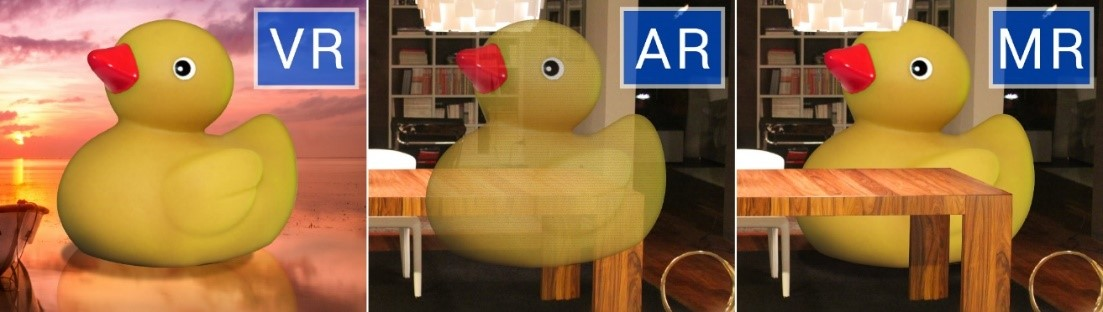
\includegraphics[scale=1.2]{differenceVrArMr.JPG}
    \caption{Visuele voorstelling verschil tussen VR, AR en MR \autocite{Barel2017}}
\end{figure}

\section{Geschiedenis}

Men zou denken dat virtual reality een relatief jonge technologie is maar niets is minder waar. De fundamenten voor VR werden al veel langer geleden vastgelegd. De beginselen van het begrip rijkt terug naar het jaar 1929. Hier werd de technologie voor de eerste keer gebruikt in een vluchtsimulator ontwikkeld door Edward Link. Deze werd gebruikt om piloten op een veilige manier op te leiden. De zogenaamde ‘Link trainer’ werd ook veel in werking gesteld gedurende de Tweede Wereldoorlog.


In de jaren ’50 ontwierp Morton Heilig de Sensorama (\textbf{figuur 2.2}). Dit was een apparaat gelijkaardig aan een grote kijkdoos die alle zintuigen stimuleerde. Wanneer men in de Sensorama plaatsnam maakte het gebruik van geuren, geluiden, beelden en trillingen om de ervaring zo realistisch mogelijk te laten lijken. 

\begin{figure}[h]
    \centering
    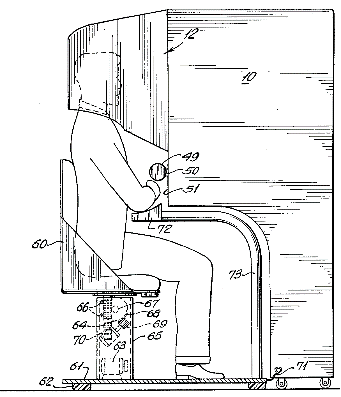
\includegraphics[scale=1]{sensorama.png}
    \caption{De sensorama ontworpen door Morton Heilig \autocite{Society2019}}
\end{figure}

In de jaren ’60 kwam Heilig met de eerste Head mounted display (HMD), Telesphere mask genoemd. Dit was het eerste voorbeeld van VR zoals we het nu kennen. Deze werkte wel nog niet met motion tracking.
Op deze functionaliteit moest men wachten tot het einde van de jaren ’60 toen ‘The ultimate display’ uit kwam.
Al deze voorgaande uitvindingen sloegen echter niet meteen aan.

Het duurde vervolgens tot in de jaren ’90 voordat de technologie weer wat relevanter werd. Hoewel het voor thuisgebruik nog steeds te duur was, konden meer en meer bedrijven het wel al aanschaffen en soms ook beschikbaar stellen voor het publiek. Op die manier kwam het beetje bij beetje al maar meer in de mainstream terecht. Enkele jaren erna sprongen grotere bedrijven zoals onder andere Nintendo mee op de VR trend en brachten VR brillen uit. De wereld was echter nog niet klaar voor Nintendo's 'virtual boy' en het draaide uit op een grote flop. 

Ook in de jaren 2000 liet virtual reality het grote publiek onverschillig achter. Het duurde totdat er in 2012 een bedrijf genaamd Oculus de Oculus Rift voorstelde op \href{https://www.kickstarter.com/}{www.kickstarter.com}, een website voor crowdfunding en startup bedrijven te financieren. De Rift kreeg veel aandacht op deze site en het startbedrag was al snel verzameld. Deze Oculus Rift (\textbf{figuur 2.3}) zou het begin zijn van het VR tijdperk dat momenteel volop in bloei staat \autocite{Society2019}.

\begin{figure}[h]
    \centering
    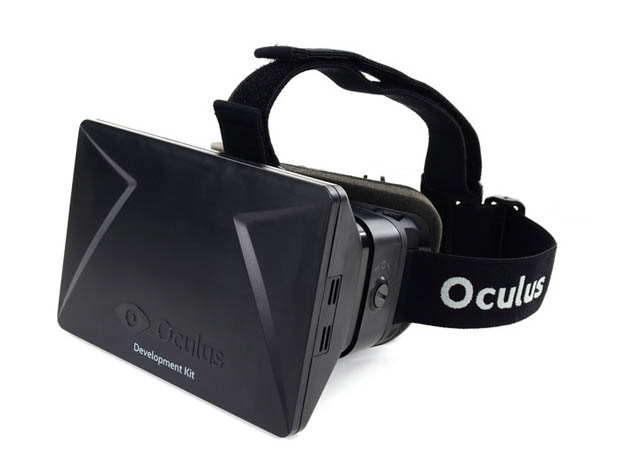
\includegraphics[scale=0.225]{oculusRift.jpg}
    \caption{De eerste Rift ontwikkeld door Oculus \autocite{Kumparak2014}}
\end{figure}

\section{Bijwerkingen}
\subsection{Misselijkheid of 'virtual reality-ziekte'}

De virtual reality ziekte is eigenlijk een vorm van bewegingsziekte of motion sickness. Andere vormen van bewegingsziekte zijn o.a. wagenziekte, zeeziekte, etc. Dit gevoel van misselijkheid is het gevolg van onduidelijke, verschillende signalen die de hersenen binnenkrijgen.

Zo zijn er in het menselijk lichaam drie systemen die ervoor zorgen dat onze positie in de ruimte berekend wordt en we bijvoorbeeld ons evenwicht kunnen houden.
Allereerst gebruiken we onze ogen om onze omgeving waar te nemen. De ogen sturen deze visuele data dan door naar de hersenen en hier wordt deze data dan verwerkt \autocite{Bovenij2019}.

Vervolgens hebben we de evenwichtsorganen waar we informatie uithalen. De evenwichtsorganen bevinden zich in het binnenoor van de gebruiker (\textbf{figuur 2.4}).

\begin{figure}[h]
    \centering
    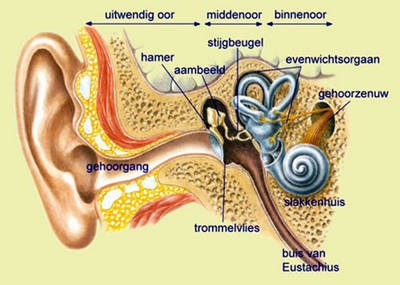
\includegraphics[scale=0.7]{binnenoor.jpg}
    \caption{Het binnenoor met het evenwichtsorgaan \autocite{Utrecht2019}}
\end{figure}

Tenslotte beschikken we ook nog over sensoren op de huid en de wervelkolom. Deze vertellen onze hersenen iets over de lichaamshouding van de persoon (\textbf{figuur 2.5}).

\begin{figure}[h]
    \centering
    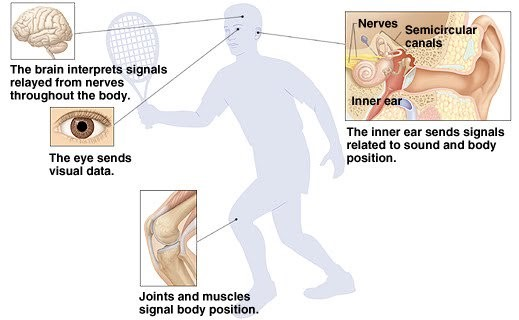
\includegraphics[scale=0.7]{sensoren.jpg}
    \caption{De sensoren van het menselijke lichaam die de hersenen info verschaffen over de positie en de verplaatsing van het lichaam in de ruimte \autocite{Dizzy2018}}
\end{figure}

Wanneer men een VR bril op het hoofd zet kan het soms gebeuren dat de hersenen verschillende signalen binnenkrijgen van de ogen en de evenwichtsorganen. De ogen zullen bijvoorbeeld denken dat men beweegt, maar de evenwichtsorganen dan weer niet. Deze verwarrende signalen zijn dan ook meteen het gevolg van de misselijkheid die men waarneemt \autocite{Kraft2017}. Dit verschijnsel komt natuurlijk, net zoals wagenziekte en zeeziekte, niet bij iedereen voor die virtual reality ervaart.

\pagebreak
De laatste jaren zijn VR ontwikkelaars al zeer gevorderd in het verminderen van motion sickness. Dit dankzij grote verbeteringen op vlak van motion tracking en het verhogen van de frame rates van de schermen die men in de headsets verwerkt. Deze factoren zorgen ervoor dat de ogen en de evenwichtsorganen meer en meer op elkaar afgesteld kunnen worden.

\subsection{Epileptische aanvallen}
Virtual reality kan ook leiden tot epileptische aanvallen bij bepaalde personen. Er wordt mensen met epilepsie dan ook afgeraden om gebruik te maken van VR headsets \autocite{Bolluyt2017}. Raadpleeg zeker eerst een arts wanneer u beslist om het toch te doen.

\subsection{Hoofdpijn en vermoeide ogen}
Wanneer men te lang naar een computer- of tv-scherm kijkt kan men soms het gevoel krijgen van vermoeide ogen en dat is bij virtual reality ook niet anders. Wat wel verschillend is bij een VR headset is dat men zich in een 3D omgeving bevindt. De ogen zullen zich dus veel frequenter moeten scherpstellen dan wanneer men naar een 2D-scherm kijkt zoals bijvoorbeeld een televisie. Daarnaast is de afstand tussen de ogen en de schermen bij VR ook kleiner. Hierdoor is de intensiteit van de lichtralen wel groter dan wanneer men naar een televisie kijkt. De ogen zullen in het algemeen dus wel sneller vermoeid raken. Vermoeide ogen kunnen soms zorgen voor een minder scherp zicht, hoofdpijn en andere kwaaltjes. Fabricanten van de headsets raden dan ook aan om regelmatig te pauzeren. De symptomen zijn echter wel slechts tijdelijk, het beste wat je kan doen is rusten. Over de effecten op lange termijn is destijds nog niet veel geweten \autocite{Bolluyt2017}.


\section{Technologieën en ontwikkelingsomgevingen}
\subsection{Game Engines}
\subsubsection{Wat is een game engine?}
Een game engine is werkelijk niets meer dan software die game developers voorziet van de nodige functionaliteiten om op een relatief snelle en efficiënte manier een game te ontwikkelen \autocite{Oculus2017}. In zo een game engine kunnen 2D-, 3D modellen en andere 'assets' ingeladen worden om de gewenste omgeving te creëren. Op die manier zijn er dus oneindig veel mogelijkheden in een game engine. Naast het feit dat men een omgeving kan opbouwen zijn er nog andere elementen waarmee men kan spelen zoals: audio, fysica, netwerkfuncties en interactie met de gebruiker. De wijze  waarop deze elementen met elkaar interageren vormen dan ook de fundamenten van het ontwikkelen van een goede game. Enkele van de meest bekende game engines zijn: Unity en Unreal game engine \autocite{Staff2018}.

\subsubsection{Unity3D}

Unity3D ofwel Unity is een zeer populaire cross-platform game engine ontwikkeld door Unity Technologies.
De eerste versie van Unity kwam in 2005 op de markt, gecreëerd door David Helgason, Joachim Ante en Nicholas Francis. Het was hun doel om een betaalbare game engine te maken die toch geavanceerde functionaliteiten te bieden had voor amateur game developers. Dit was dan ook een van de grootste redenen dat Unity later zo populair werd. Omdat ze geïnspireerd waren door de eenvoudige workflow van Apple programma's was hun eerste versie dus ook enkel toegankelijk voor Mac gebruikers. Hun échte doorbraak kwam echter pas in 2008, gevolgd door het ontstaan van de Apple Iphone en daarbij ook de Apple Appstore. Unity besloot toen om een toegankelijke versie te maken om applicaties voor Iphone's te ontwikkelen. Na hun grote succes op IOS werd het duidelijk dat ze ook een versie voor Windows nodig hadden. Wat Unity vandaag de dag nog steeds zeer populair maakt is het cross-platform element. Momenteel ondersteunt Unity vier categorieën: mobile, web, console en computer. Men kan m.b.v. Unity dus bijna alle publieken bereiken \autocite{Haas2014}.

\subsubsection{Unreal Engine}
Naast Unity hebben we nog een andere veel gebruikte game engine nl. Unreal engine. Deze game engine werd ontwikkeld door Epic Games en werd voor de eerste keer voorgesteld bij de release van de populaire shooter game Unreal in 1998. Deze engine werd vooral gebruikt door de grotere game ontwikkelaars en -studio's. Het was minder populair bij de amateur ontwikkelaar omdat men een abonnement nodig had om toegang te krijgen. Vandaag de dag is Unreal Engine echter volledig gratis \autocite{Sutorcen2016}.

\subsection{Degrees of freedom}

Een belangrijke eigenschap van een VR headset zijn zijn vrijheidsgraden ofwel degrees of freedom (DOF). Dit slaat op het aantal verschillende richtingen dat een object kan bewegen in een 3D wereld. Er bestaan twee soorten vrijheidsgraden in VR: 3 DOF en 6 DOF. 

\subsubsection{3 degrees of freedom}
Bij 3 degrees of freedom kan een VR headset enkel de hoofdbeweging tracken, het systeem zal dus weten welke kant je opkijkt. Bij een 3 DOF headset kan men dus bewegen volgens drie assen genaamd: roll, yaw en pitch (\textbf{figuur 2.6}). Men kan dus stellen dat hier de oriëntatie getrackt wordt maar de positie niet. In een virtuele omgeving zal de gebruiker dus enkel kunnen 'rondkijken' terwijl hij steeds op dezelfde plaats blijft staan. De reden waarom men vaak nog 3 DOF gebruikt is omdat het heel eenvoudig is om enkel de oriëntatie te tracken. Zo zitten er in elke smartphone al voldoende sensoren om dit te tracken nl. een accelerometer en een gyroscoop. De positie in de ruimte tracken is echter al veel lastiger \autocite{Weis2018}.

\begin{figure}[h]
    \centering
    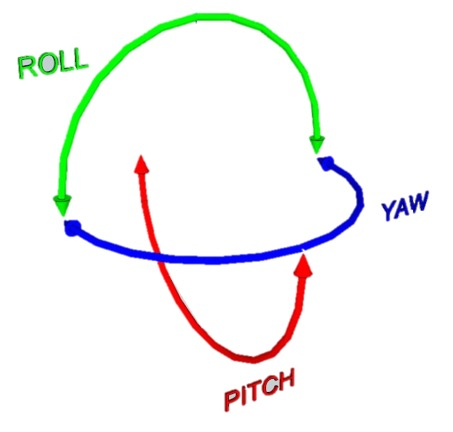
\includegraphics[scale=0.35]{3dof.jpg}
    \caption{De 3 assen voor oriëntatie te tracken: roll, yaw en pitch \autocite{Lang2013}}
\end{figure}

\subsubsection{6 degrees of freedom}
Wanneer men een 6 DOF headset gebruikt voelt men meteen dat de ervaring meer natuurlijk is dan een 3DOF systeem. Bij dit systeem wordt dus niet enkel de oriëntatie getrackt maar daarnaast ook de positie in de ruimte (\textbf{figuur 2.7}). Deze positie wordt eveneens door 3 assen bepaald nl. x-as, y-as en z-as. Hier zal de gebruiker in de virtuele omgeving naast rondkijken dus ook kunnen rondlopen zoals in de realiteit. Op hedendaagse headsets wordt het tracken van de positie meestal gerealiseerd door sensoren op de headset of externe camera's \autocite{Weis2018}.

\begin{figure}[h]
    \centering
    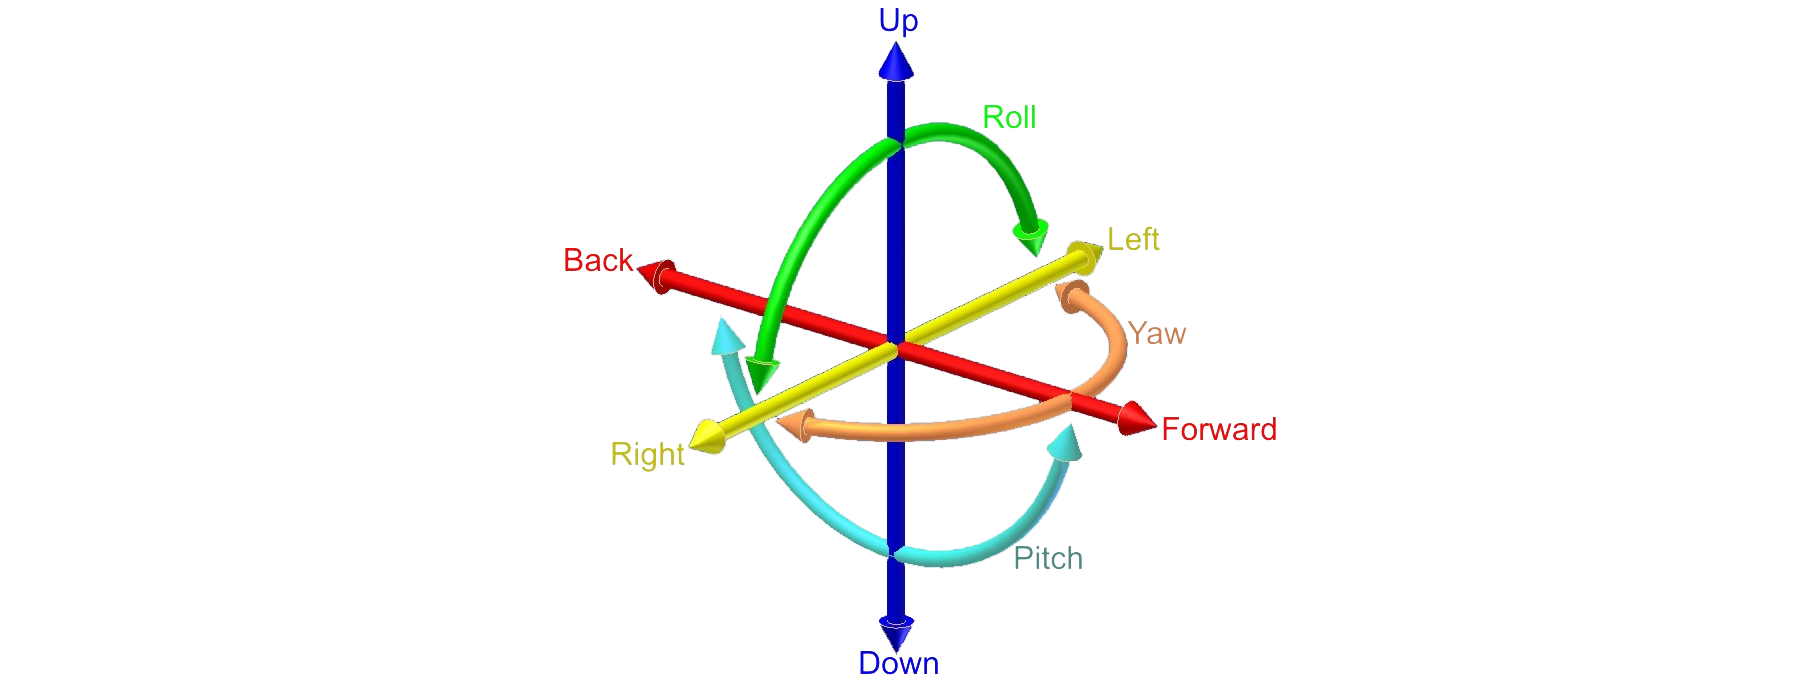
\includegraphics[scale=0.25]{dofAxis.png}
    \caption{De 6 assen voor oriëntatie en positie te tracken: roll, yaw, pitch, x-as, y-as en z-as \autocite{Weis2018}}
\end{figure}

\pagebreak

\section{Verschillende soorten VR headsets}

\subsection{Desktop VR}
Bij desktop VR headsets dient men steeds verbonden te zijn met een krachtige computer. Andere benamingen voor deze soort headsets zijn 'room-scale VR' of 'tethered VR', dat laatste wijst dus op de kabels die steeds nodig zijn om verbonden te zijn met een computer. Het voordeel van deze soort headsets is dat het momenteel de grootste immersie aan de gebruiker kan leveren. Dit komt door de grote rekenkracht van de PC waardoor er veel kwaliteitsvollere omgevingen gerenderd kunnen worden, het aantal frames per seconde hoger ligt, etc. Ook beschikken de meeste desktop VR headsets over 6 degrees of freedom (6 DOF). Het nadeel is zoals eerder al genoemd dat men steeds vasthangt aan een externe computer en daarnaast zijn de instapkosten nog redelijk prijzig \autocite{Cherdo2018}. Enkele bekende desktop VR headsets zijn: Oculus Rift, HTC Vive (\textbf{figuur 2.8}) en de HTC Vive Pro.

\begin{figure}[h]
    \centering
    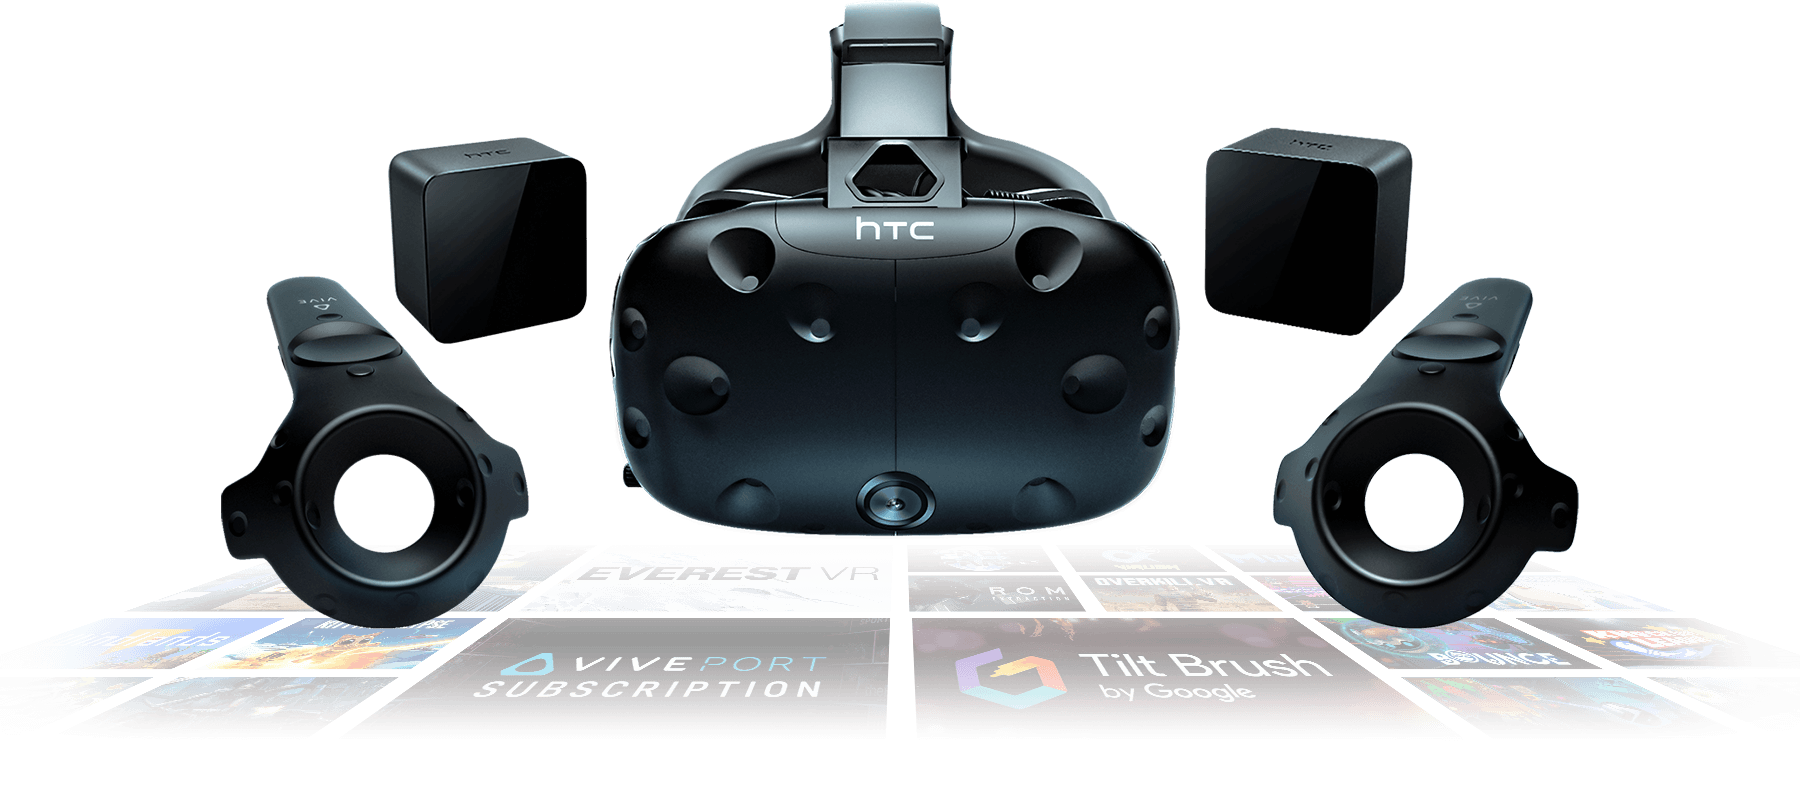
\includegraphics[scale=0.14]{vive.png}
    \caption{De HTC Vive desktop VR headset \autocite{Vive2019}}
\end{figure}


\subsection{Mobile VR}
Door de grote opmars van de smartphone de laatste jaren hebben veel bedrijven zich eerst gericht op mobile VR. Iedereen had plots toegang tot VR en dit zorgde dan ook voor een grote interesse bij de mainstream. Bij een mobile headset wordt er dus eenvoudigweg een smartphone in een headset geplaatst.
Een smartphone heeft in principe dus alles wat nodig is om te dienen als aandrijver van een VR headset. Het voordeel bij deze soort headsets is dat men geen kabels nodig heeft dus overal kan genieten van de VR ervaring. Helaas is er wel een keerzijde, namelijk dat een smartphone de rekenkracht van een externe computer niet kan bijhouden. Mobile VR zal (momenteel) dus steeds wat minder immersive aanvoelen dan een desktop VR. Daarnaast beschikt een smartphone enkel over sensoren om voor een 3 DOF ervaring te zorgen \autocite{Cherdo2018}.
Enkele bekende mobile headsets zijn: Samsung Gear VR, Google Daydream en Google cardboard.

\subsection{Standalone VR}
Bij deze soort headsets heeft men geen externe computer of smartphone nodig, alles zit erin (all-in-one). Deze categorie vormt de gulden middenweg tussen de twee vorige categorieën. Aan de ene kant hoeft men geen kabels in te steken alvorens men aan de slag kan gaan. Aan de andere kant zijn deze standalone's ook meer geschikt voor VR dan smartphones. Bij een standalone hangt men bijvoorbeeld niet vast aan de 3 DOF, men kan in de headset sensoren integreren zodat men een 6 DOF headset kan verkrijgen  \autocite{Cherdo2018}. Voorlopig zijn er enkel nog maar 3 DOF standalone headsets ter beschikking voor het grote publiek, de meest bekende is de Oculus Go. Ditzelfde bedrijf heeft echter al een 6 DOF standalone headset aangekondigd, Oculus Quest genaamd (\textbf{figuur 2.9}). Deze headset beschikt over 6 degrees of freedom, tracked controllers voor beide handen en daarnaast is hij out of the box meteen gebruiksklaar \autocite{Oculus2019}. Dit zijn dan ook enkele redenen waarom deze nieuwe headset zeker zal aanslaan bij het grote publiek.

\begin{figure}[h]
    \centering
    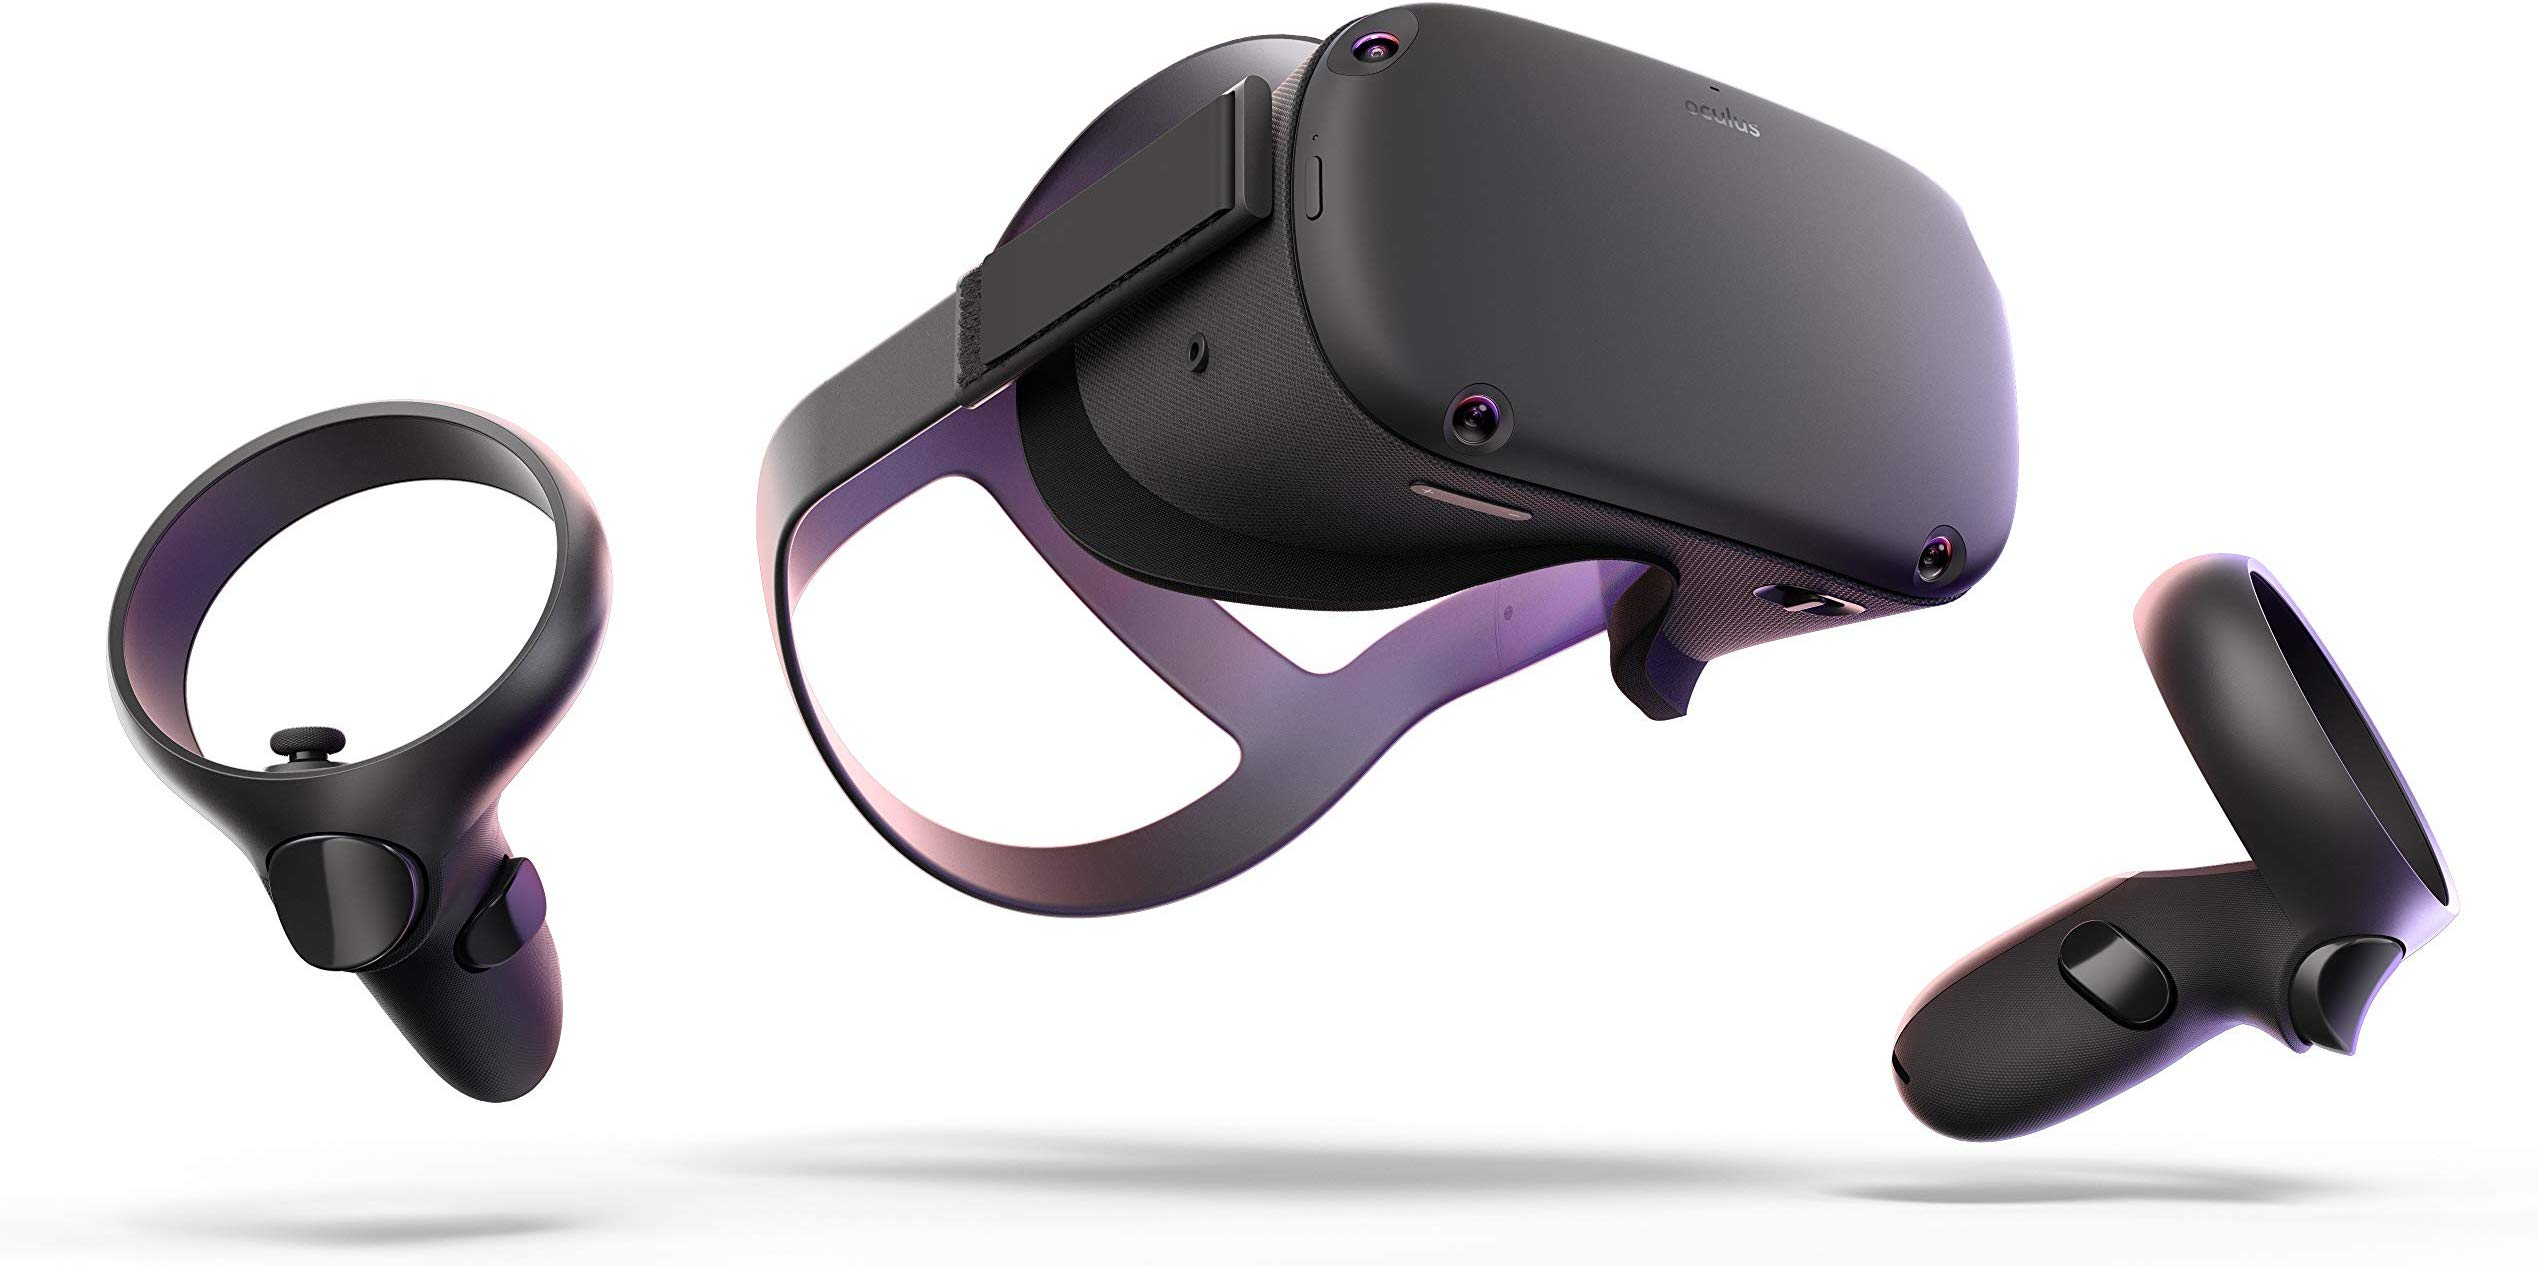
\includegraphics[scale=0.1]{quest.jpg}
    \caption{De Oculus Quest 6DoF standalone headset \autocite{Oculus2019}}
\end{figure}


\chapter{VR in de gezondheidszorg}
\section{Inleiding}
Nadat in het vorige hoofdstuk het begrip'Virtual reality' werd aangekaard, zal men in dit hoofdstuk meer ingaan op VR in de gezondheidszorg. Er zullen een aantal actuele use cases van VR behandeld worden. Verder wordt er ook dieper ingegaan op de revalidatiesector en enkele bestaande applicaties.

\section{Actuele use cases}
\subsection{Simulatie van behandelingen en operaties}
VR zorgt momenteel al voor grote doorbraken op educatief vlak in de gezondheidszorg. Zo bestaan er al applicaties waar studenten in een virtuele omgeving worden getraind om operaties uit te voeren. Op deze wijze kan een student leren uit zijn/haar fouten zonder cruciale gevolgen (\textbf{figuur 3.1}). Door operaties al in de praktijk te oefenen stimuleert men het visuele en het fysieke geheugen dat ervoor zorgt dat de handelingen beter onthouden worden. Daarnaast kan virtual reality ook de kosten van training in de gezondheidszorg verlagen. Zo kunnen er meer mensen tegelijk opgeleid worden en moet men niet herhaaldelijk materiaal aankopen voor een bepaalde operatie \autocite{Elion2018}.

In 2017 werkte Oculus samen met CHLA, een kinderziekenhuis in Los Angeles, om een dergelijke training applicatie te ontwikkelen. Studenten worden er blootgesteld aan stressvolle situaties terwijl ze snel beslissingen moeten nemen om een patiënt in leven te houden \autocite{Adobe2018}.

\begin{figure}[h]
    \centering
    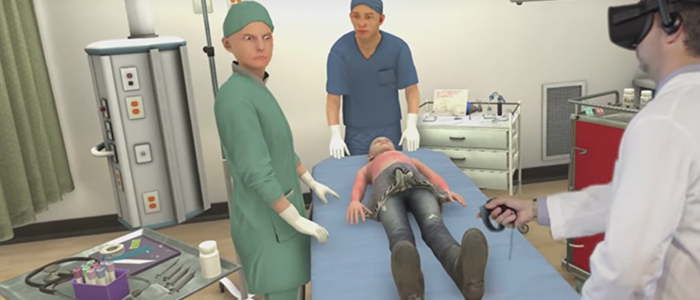
\includegraphics[scale=0.4]{healthApp.jpg}
    \caption{VR simulatie app ontwikkeld door Oculus waar de gebruiker in een gesimuleerde noodsituatie terecht komt \autocite{Adobe2018}}
\end{figure}

Dr. Shafi Ahmed voerde in 2016  als één van de eersten een operatie uit op een gezwel in de darm van een kankerpatiënt terwijl hij deze beelden live uitzond in VR (\textbf{figuur 3.2}). Op deze manier konden studenten de procedure op de voet volgen alsof ze zelf in de kamer stonden \autocite{Pelta2017}.

\begin{figure}[h]
    \centering
    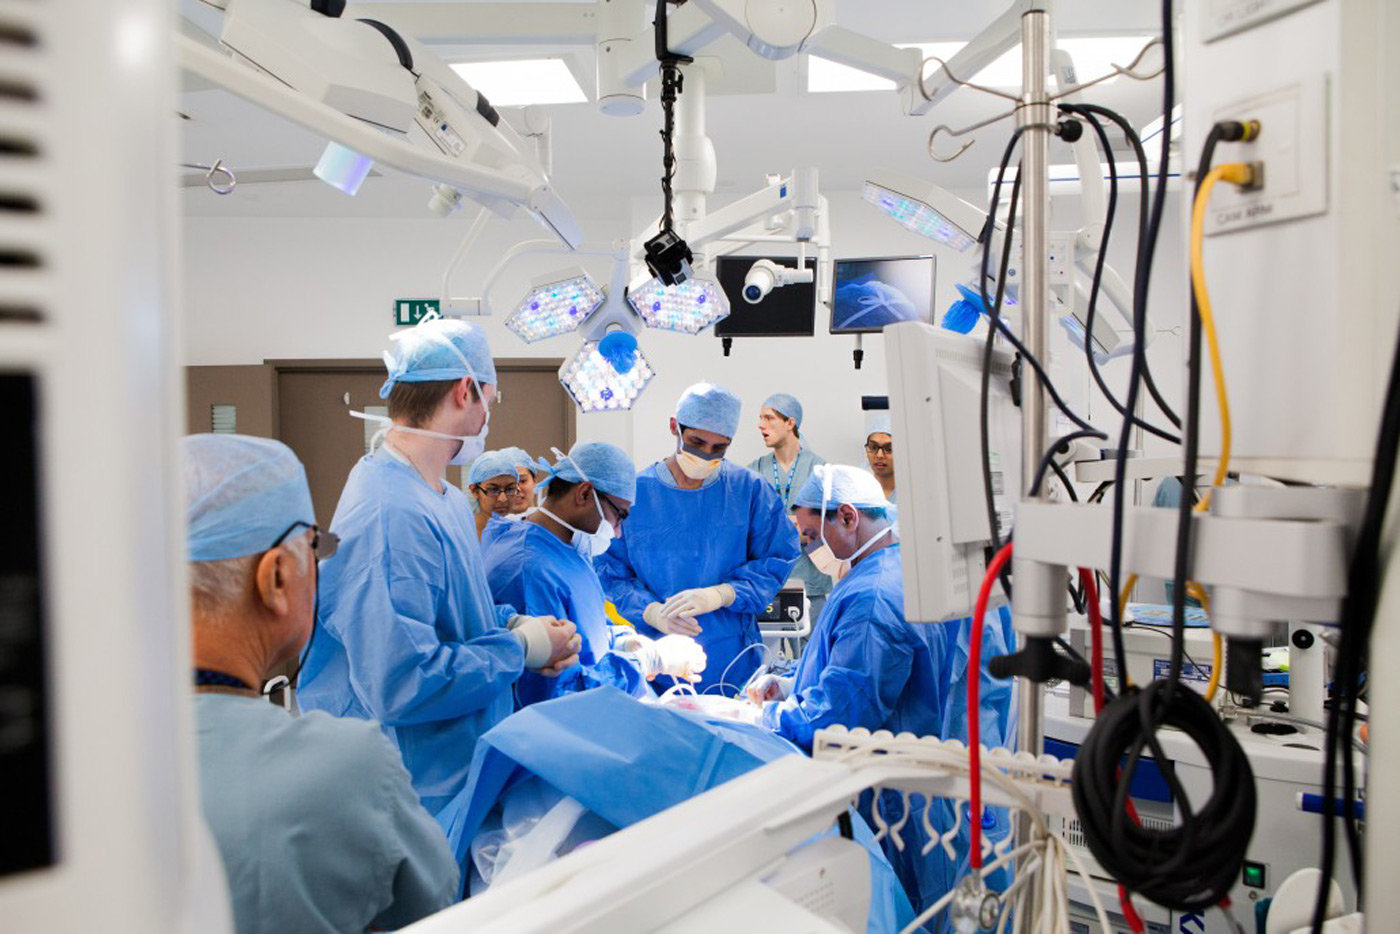
\includegraphics[scale=0.18]{vrOperatie.jpg}
    \caption{Dr. Shafi Ahmed zendt zijn operatie live uit a.d.h.v 360-graden camera's \autocite{Realities2019}}
\end{figure}

\subsection{Stress- en angstbeheersing}  
Bij behandeling van angststoornissen in de psychiatrie wordt er vaak gebruik gemaakt van ‘exposure therapie’. Hierbij wordt een persoon geleidelijk blootgesteld aan het gevreesde object of situatie. Dit gebeurt wel op een gecontroleerde manier en in een veilige omgeving waardoor de patiënt gedwongen wordt om zijn angst onder ogen te komen in plaats ervan te vluchten. Deze methode wordt dan toegepast totdat de angst beheersbaar is \autocite{Keller2018}. 

Bij traditionele methoden ging men een patiënt met arachnofobie bijvoorbeeld blootstellen aan foto’s, video’s en figuren van spinachtigen. Het nadeel bij deze methode is wel dat een persoon nog altijd die barrière ervaart tussen de realiteit en zijn angst waardoor deze minder effectief wordt \autocite{Keller2018}.

Een andere methode is de in-vivo methode waar de patiënt in werkelijkheid wordt blootgesteld aan zijn angst. Bijvoorbeeld iemand met vliegangst die werkelijk op een vliegtuig stapt en zo aan zijn angst wordt blootgesteld. Het nadeel aan deze methode is dat het voor sommigen een te grote stap is om meteen te overwinnen. Daarnaast kan een in-vivo methode ook snel kostelijk worden \autocite{Keller2018}.

VR elimineert dus een mogelijke barrière voor patiënten die problemen kunnen ondervinden met het inbeelden of visualiseren van de angst. Ook zal een VR methode in vele gevallen kostenbesparender zijn dan bepaalde in-vivo methoden \autocite{Keller2018}.

Virtual reality wordt dan ook heel vaak gebruikt om deze soorten therapieën uit te voeren. Virtuele omgevingen kunnen aangemaakt worden die de patiënt stapsgewijs aan de gevreesde factor blootstellen \autocite{Keller2018}.

Naast angststoornissen is VR ook heel effectief bij stressbeheersing. Stress en burn-outs worden al maar grotere factoren op de werkplaats en bedrijven proberen er dan ook beter op in te spelen. Zo zou een werknemer die een grote werkdruk en stress ervaart ook minder productief zijn doorheen zijn/haar werkdag. Daarom stelt men in sommige organisaties VR headsets ter beschikking voor werknemers om te ‘ontstressen’ \autocite{Thoondee2017}.  
Zo een ontspannende applicatie bestaat dan uit een relaxerende virtuele omgeving zoals bijvoorbeeld natuuromgevingen, meditatieruimte, etc.

\subsection{Efficiëntere revalidatie na beroerte}  
De laatste jaren is het gebruik van virtual reality bij patiënten die een beroerte gekend hebben al maar toegenomen. Na een beroerte kan men in de hersenen nieuwe neurale verbindingen vormen door veel taakgerichte oefeningen uit te voeren. Op deze manier kan men de hersenen als het ware 'herprogrammeren'. Deze nieuwe verbindingen stimuleren het herstel van motorische vaardigheden bij patiënten na een beroerte. \textcite{Laver2017} vergeleek in 2017 de effecten van gebruikelijke therapie met de effecten van virtual reality bij de bovenste ledematen. Men concludeerde hier dat VR leidde tot verbeteringen in het uitvoeren van dagelijkse taken. Echter was het wel nog niet duidelijke of deze effecten blijvend waren \autocite{Laver2017}.

\section{Mirror therapy}
Spiegeltherapie ofwel mirror therapy is een revalidatie methode die voor het eerst werd gebruikt in 1995 door dr. Ramachandran, een Amerikaanse neuroloog. Het principe van de methode is dat men door het gebruik van een spiegel de beweging van een verlamd of geamputeerd ledemaat kan veinzen voor het brein waardoor men de hersenen als het ware opnieuw kan programmeren \autocite{Physiopedia2019}.
Een patiënt voert dus oefeningen uit met het functionerende ledemaat, maar door de spiegel lijkt het alsof het niet functionerende ledemaat de oefeningen ook uitvoert (\textbf{figuur 3.3}).

\subsection{Neuroplasticiteit}
De plasticiteit van een neuron verwijst naar zijn vermogen om te veranderen. Elke keer dat je een beweging maakt of je hersenen denken dat je een beweging maakt, bouwt het brein verbindingen op, neurale verbindingen. Wanneer iemand bijvoorbeeld verlamd raakt aan zijn/haar arm betekent dat dat er neurale verbindingen verbroken zijn die de patiënt toelaat om deze beweging uit te voeren. Doordat een patient m.b.v een spiegel het brein dus kan misleiden, worden er bij elke beweging die men doet met het functionerende lidmaat nieuwe verbindingen gelegd voor het verlamde lidmaat in de hersenen \autocite{Saebo2018}.

\subsection{Toepassingen van mirror therapy}
Een van de toepassingen waar mirror therapy bijvoorbeeld vaak gebruikt wordt is tijdens het revalidatieproces van een beroerte.  Vele mensen die een beroerte beleefd hebben blijven halfzijdig verlamd achter. Dit komt doordat de hersenen in bepaalde gebieden, die instaan voor de besturing van bepaalde ledematen, beschadigd zijn. Door gebruik te maken van mirror therapy worden er in de hersenen nieuwe neurale verbindingen gelegd voor het verlamde ledemaat \autocite{Rehab2018}. Een veelgebruikt instrument voor de uitvoering van deze methode is een “mirror box”. Zo een box heeft een driehoekige vorm en de patiënt is in staat om zijn verlamde ledemaat er in te laten rusten. Op die manier wordt het brein er minder visueel mee geconfronteerd.

Een andere toepassing van mirror therapy is bij het behandelen van fantoompijn. Wanneer men door amputatie de zenuwen van het lidmaat naar de hersenen doorbreekt vindt er geen informatieverkeer meer plaats. Door deze plotse verandering en het wegvallen van een bepaalde input zal het gebied in de hersenen overgevoelig worden en pijnprikkels kunnen creëren. Door middel van mirror therapy zal men dit gebied dus weer wat kunnen activeren en de pijn zal dus afnemen \autocite{Veenstra2019}.

Tot slot wordt mirror therapy ook gebruikt bij het verminderen van kinesiofobie of bewegingsangst. Kinesiofobie komt bij vele (vooral chronische) patiënten voor en wordt veroorzaakt doordat het brein een bepaalde beweging gaat linken aan pijn. De patiënt zal hierdoor de beweging vaak niet durven uitvoeren door angst voor deze pijn \autocite{KOCHOA2019}. De uitdaging voor de kinesist bestaat erin om het vertrouwen van de patiënt te winnen zodat de beweging toch volbracht kan worden. Een andere optie is het gebruik maken van een spiegeltherapie. Door de spiegel te gebruiken tijdens de uitvoering van de oefeningen worden de hersenen misleid en opnieuw getraind. Op die manier zal de patiënt de beweging minder linken aan pijn en zal de oefening efficiënter uitgevoerd kunnen worden \autocite{Burken2019}.

Hoewel deze alternatieve revalidatie methode dus al regelmatig wordt toegepast en het al vele patiënten succesvol heeft geholpen is men momenteel nog bezig met wetenschappelijk de effectiviteit ervan te onderzoeken.

\begin{figure}[h]
    \centering
    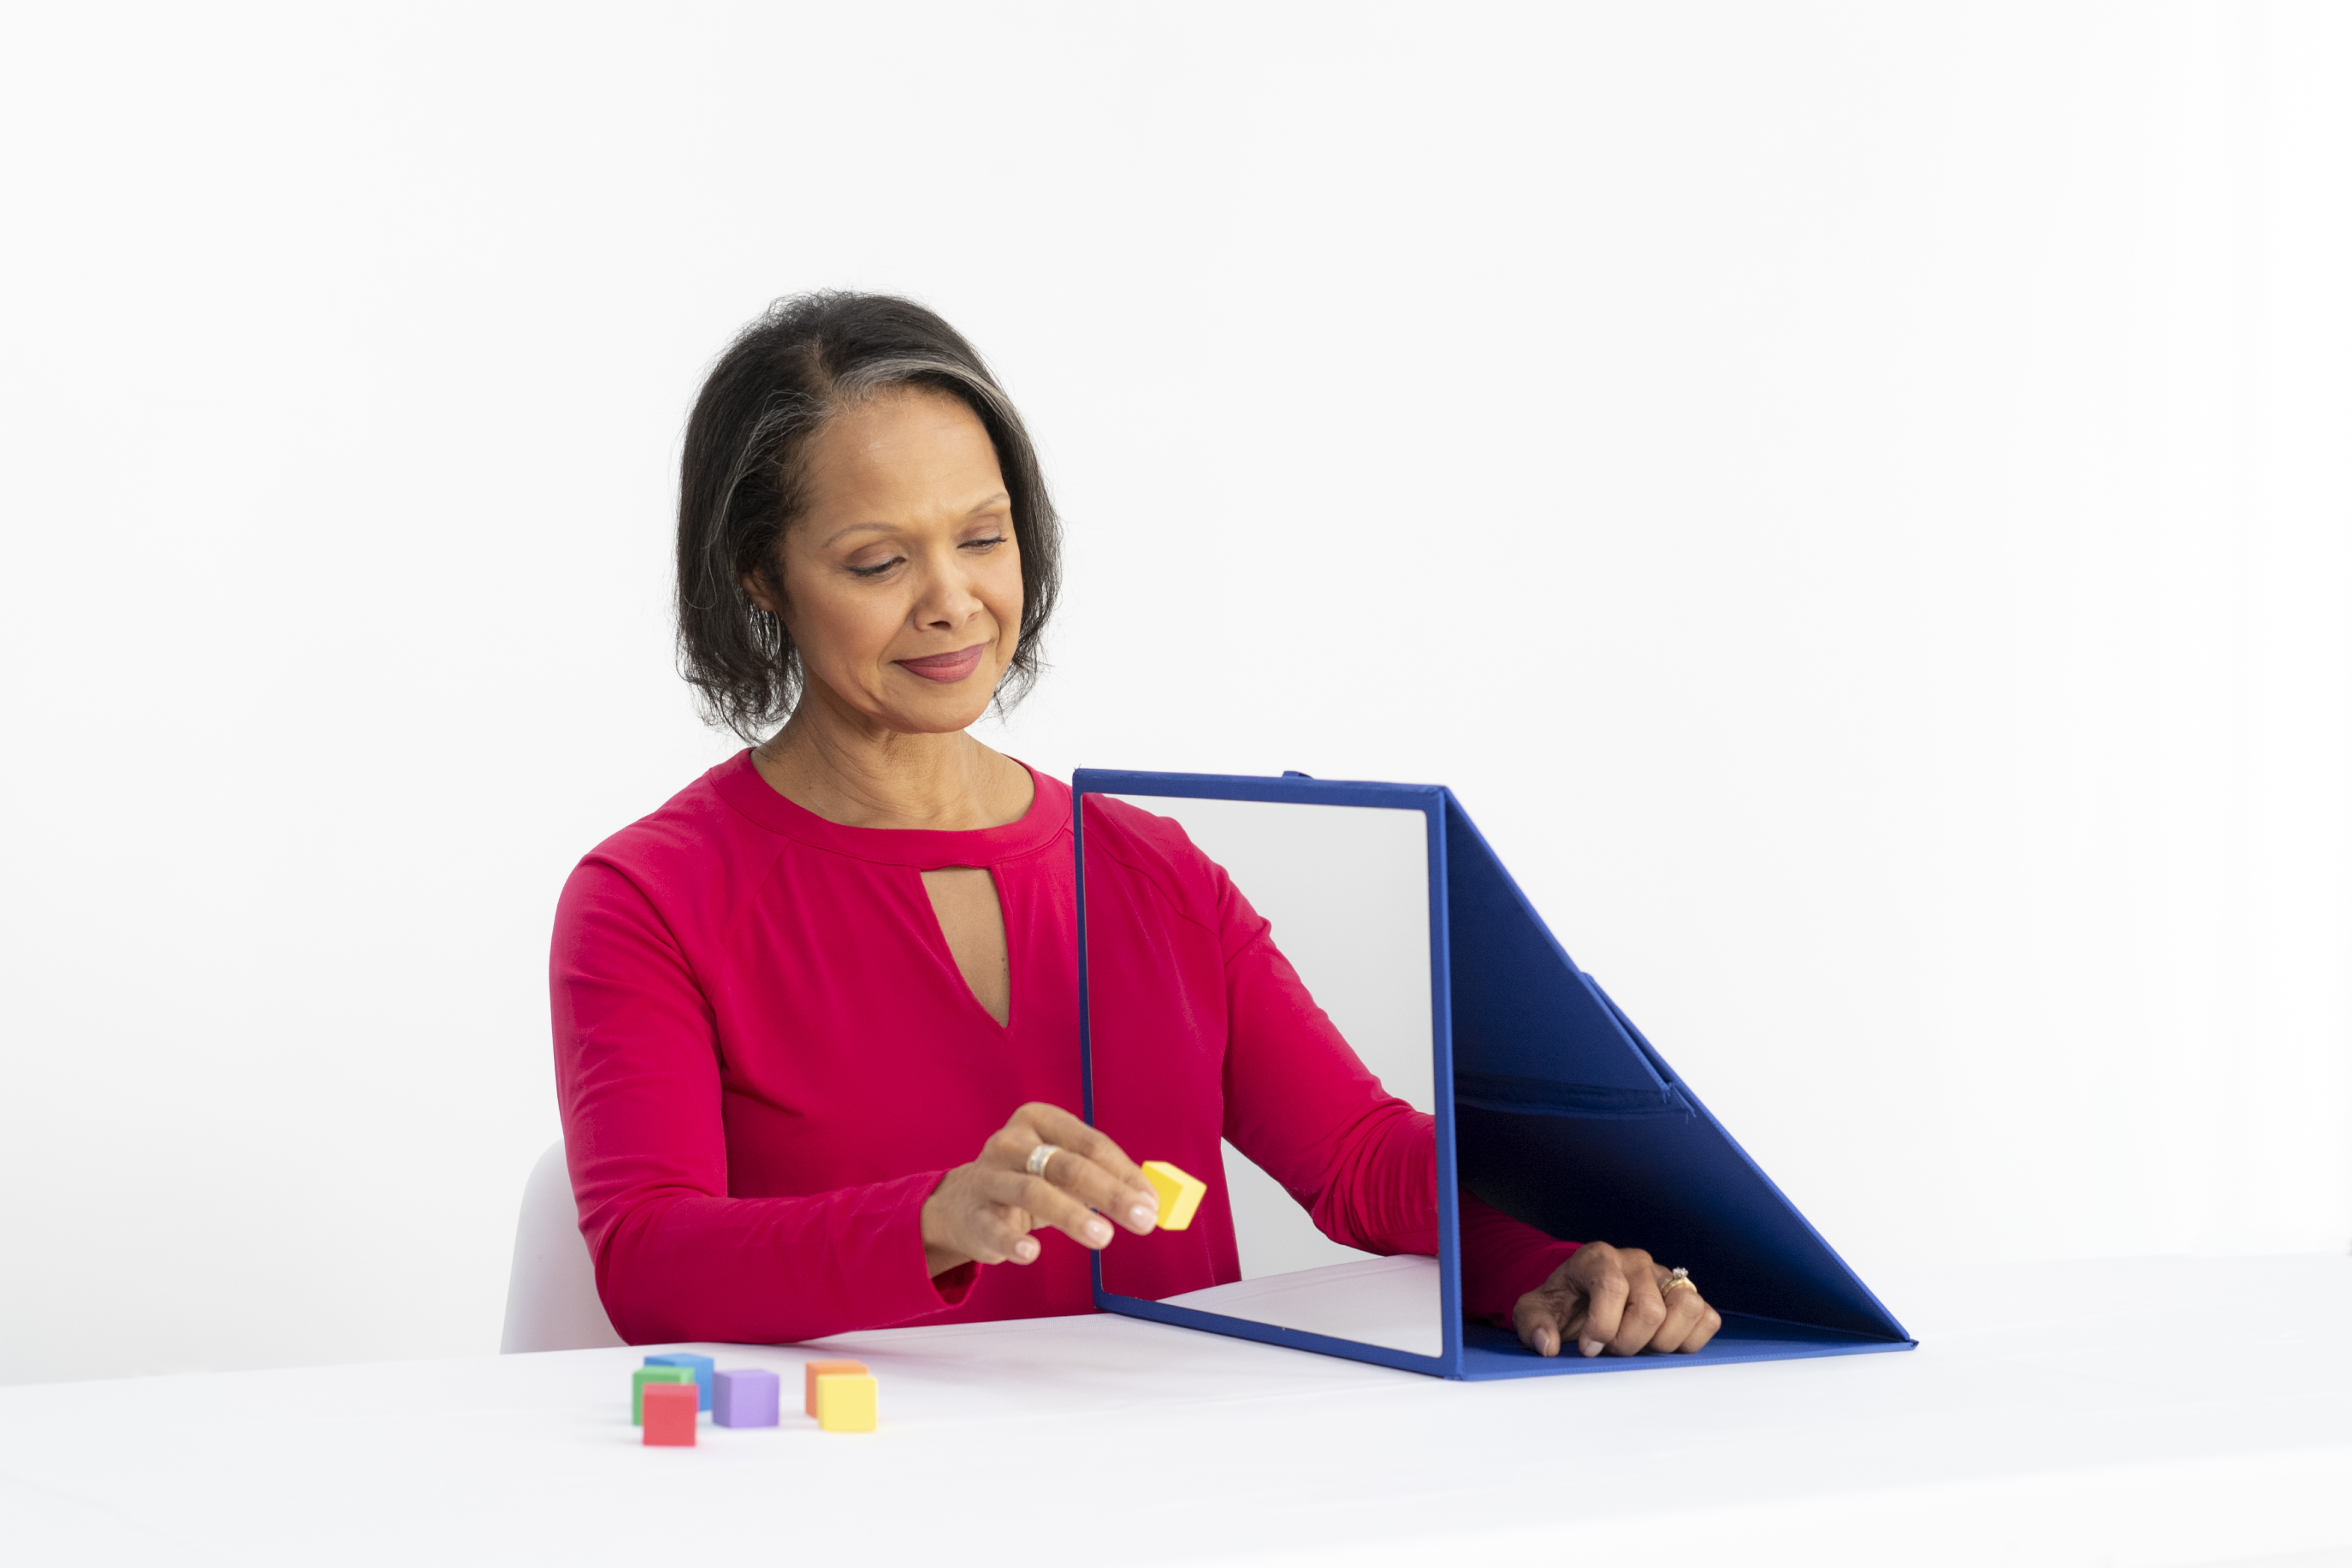
\includegraphics[scale=0.06]{mirrorTherapy.jpg}
    \caption{De mirror box in gebruik voor een verlamde arm \autocite{Saebo2018}}
\end{figure}

\subsection{VR mirror therapy}
Momenteel zijn er al enkele applicaties op de markt die mirror therapy ook mogelijk maken in VR omgevingen. Wanneer de gebruiker bijvoorbeeld bewegingen uitvoert met zijn rechtse hand zal dit in de virtuele omgeving vertaalt worden naar bewegingen met de linker hand. Een mogelijke hypothese zou zijn dat VR mirror therapy meer kans heeft om resultaten op te leveren omdat de beleving veel echter lijkt dan bij een spiegel. Momenteel is er hier echter ook nog geen wetenschappelijk bewijs voor dat dit effectiever zou zijn dan de mirror box methode of andere traditionele methodes. 

\section{Distraction therapy}
Het principe van distraction therapy is dat men de aandacht van de patiënt gaat afleiden. Men wordt afgeleid van bepaalde onaangename stimuli en in plaats daarvan wordt er meer focus gelegd op aangenamere stimuli. Dit resulteert in een vermindering van de waarneming van pijn. 

\begin{figure}[h]
    \centering
    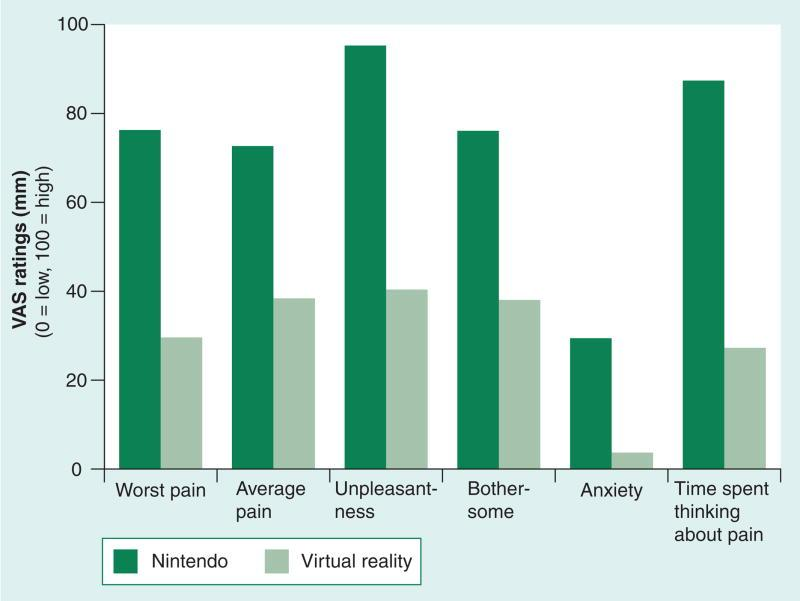
\includegraphics[scale=0.57]{painRelief.jpg}
    \caption{ Verschil in pijnervaring zonder VR en met VR tijdens het verzorgen van brandwonden \autocite{Panjwani2017}}
\end{figure}

\newpage

Een voorbeeld van distraction therapy m.b.v. VR is de game “Snowworld”, een game die vooral gericht was op patiënten met brandwonden. In deze game kwam men terecht in een sneeuwlandschap en kon men sneeuwmannen bekogelen met sneeuwballen. Dit idee kwam er doordat dergelijke patiënten vaak nog een brandende pijn voelen bij het behandelen van hun wonden. Door de focus op ijzige en sneeuwachtige landschappen te leggen zouden de patiënten minder pijnprikkels ervaren \autocite{Panjwani2017} .
Hoffman voerde hier een experiment naar uit en bij alle patiënten resulteerde het gebruik van VR in een verminderde ervaring van pijn. Daarnaast vergelijk hij ook de verschillen in pijnervaring tussen een non-VR en een VR game, de resultaten zijn terug te vinden in \textbf{figuur 3.4}. Ook hier waren de verschillen bij de proefpersonen significant. Op \textbf{figuur 3.5} zijn ook opmerkelijke verschillen terug te vinden in pijngerelateerde hersenactiviteit.

\begin{figure}[h]
    \centering
    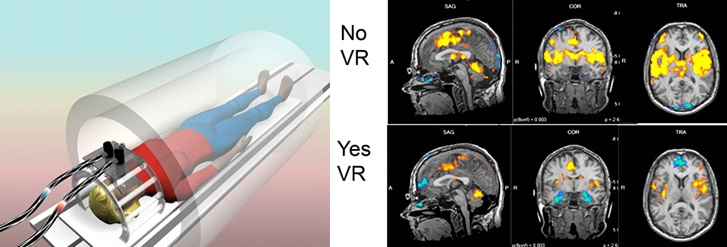
\includegraphics[scale=0.7]{distractionScan.jpg}
    \caption{MRI-hersenscans tonen significante verminderingen van pijngerelateerde hersenactiviteit tijdens SnowWorld \autocite{Washington2017}}
\end{figure}

\section{Soortgelijke applicaties}
\subsection{Mindmotion}
Mindmaze is een Zwitsers bedrijf dat zich bezighoudt met de neurorevalidatie van een patiënt na een beroerte. Ook hier wordt er geprobeerd om de patiënt op een speelse manier te laten revalideren en op die manier de motivatie bij de patiënt hoog te houden. Momenteel beschikt het bedrijf over twee producten namelijk de Mindmotion Pro en de Mindmotion Go. Zoals de naam al prijsgeeft is de Mindmotion pro (\textbf{figuur 3.6}) hun paradepaardje. Deze kan immers heel snel ingezet worden bij een patiënt na het oplopen van een letsel. Daarnaast ondersteunt het ook nog eens mirror therapy wat de neurorevalidatie dus zeker bevordert. Dit product maakt echter nog geen gebruik van virtual reality \autocite{Mindmotion2019}.

\begin{figure}[h]
    \centering
    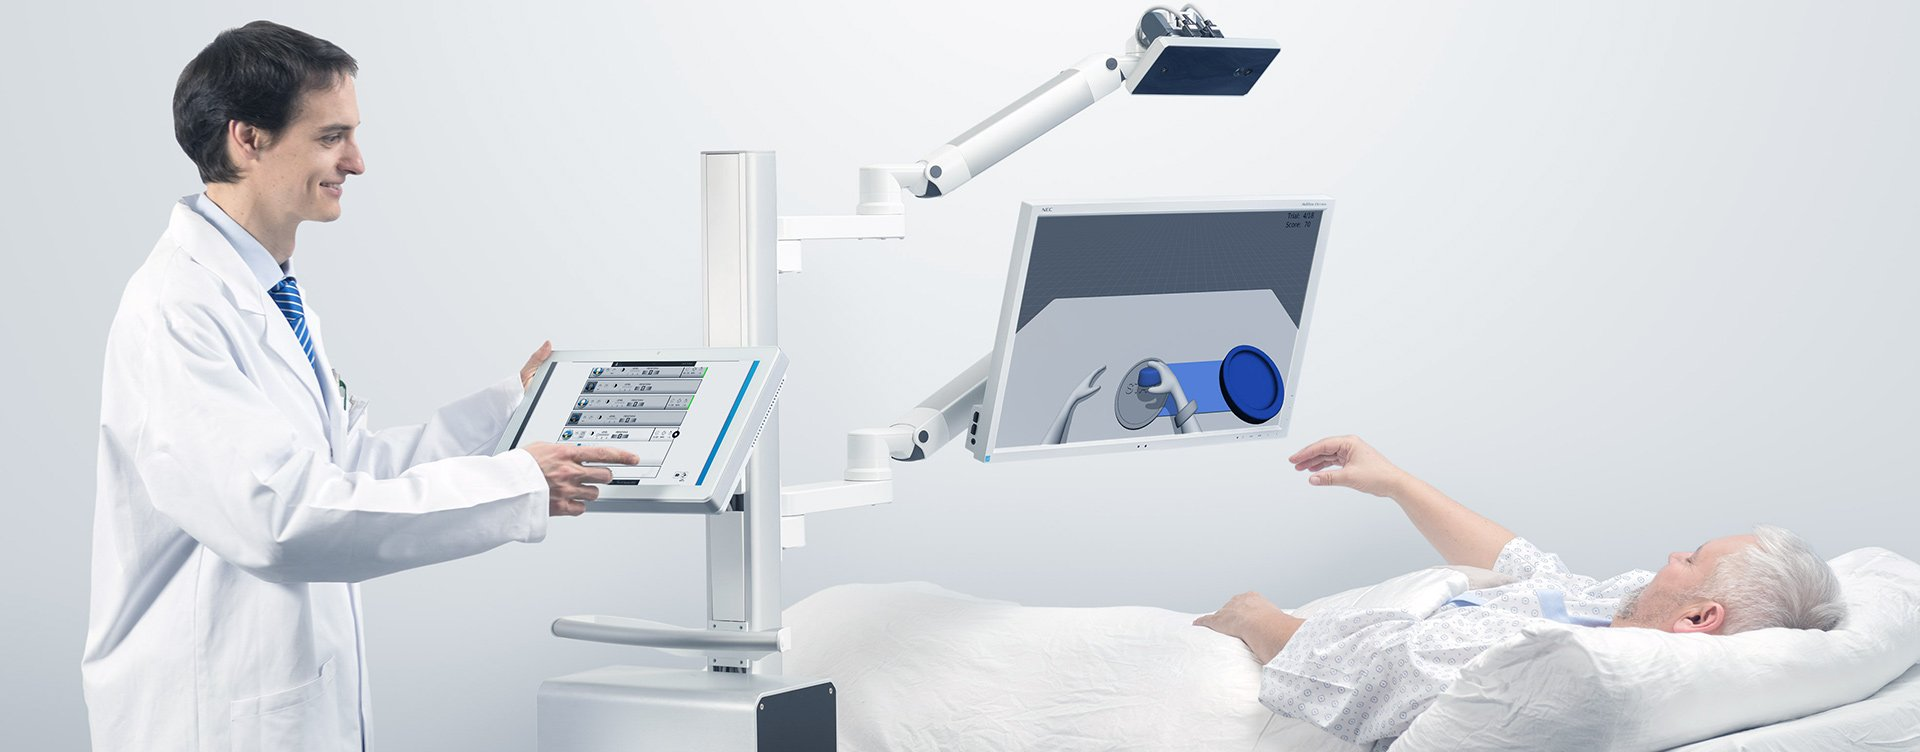
\includegraphics[scale=0.17]{mindmotion.jpg}
    \caption{Mindmotion Pro in gebruik \autocite{Mindmotion2019}}
\end{figure}

\subsection{XRHealth}
XRHealth is een applicatie die zeer gelijkt op het idee achter deze scriptie. Gebruikers komen in deze applicatie terecht in een virtuele wereld waar ze d.m.v. games hun revalidatie oefeningen uitvoeren. Wat VRHealth bijzonder maakt is dat het zich focust op gebruik in de gezondheidszorg specifiek. De applicatie laat een kinesist bijvoorbeeld toe om de resultaten en de vooruitgang van een patiënt op te volgen. In deze organisatie maakt men vooral gebruik van de Oculus Go wat zich classificeert als standalone headset. Het nadeel hiervan is dat het maar beschikt over 3 degrees of freedom en het slechts één controller bevat om handbewegingen te tracken. Bij VRHealth draait het dus vooral om de revalidatie van de bovenste lidmaten \autocite{XRHealth2019}. 

\subsection{KineQuantum}
Tot slot is er ook een bedrijf genaamd KineQuantum dat, net zoals VRHealth, zich focust op de revalidatie van patiënten m.b.v. virtual reality. Opnieuw kan de kinesist hier ook de resultaten en de vooruitgang van de patiënt opvolgen via de computer \autocite{KineQuantum2019}. Wat KineQuantum wel onderscheidt van organisaties zoals VRHealth is dat ze te werk gaan met Desktop VR headsets (\textbf{figuur 3.7}). De desktop headsets zullen dus betere tracking hebben van de bewegingen van de patiënt en beschikken over 6 degrees of freedom waar de standalone headsets voorlopig maar 3 degrees of freedom zullen halen. Het nadeel ervan is echter wel dat er steeds een computer aanwezig moet zijn. 

\begin{figure}[h]
    \centering
    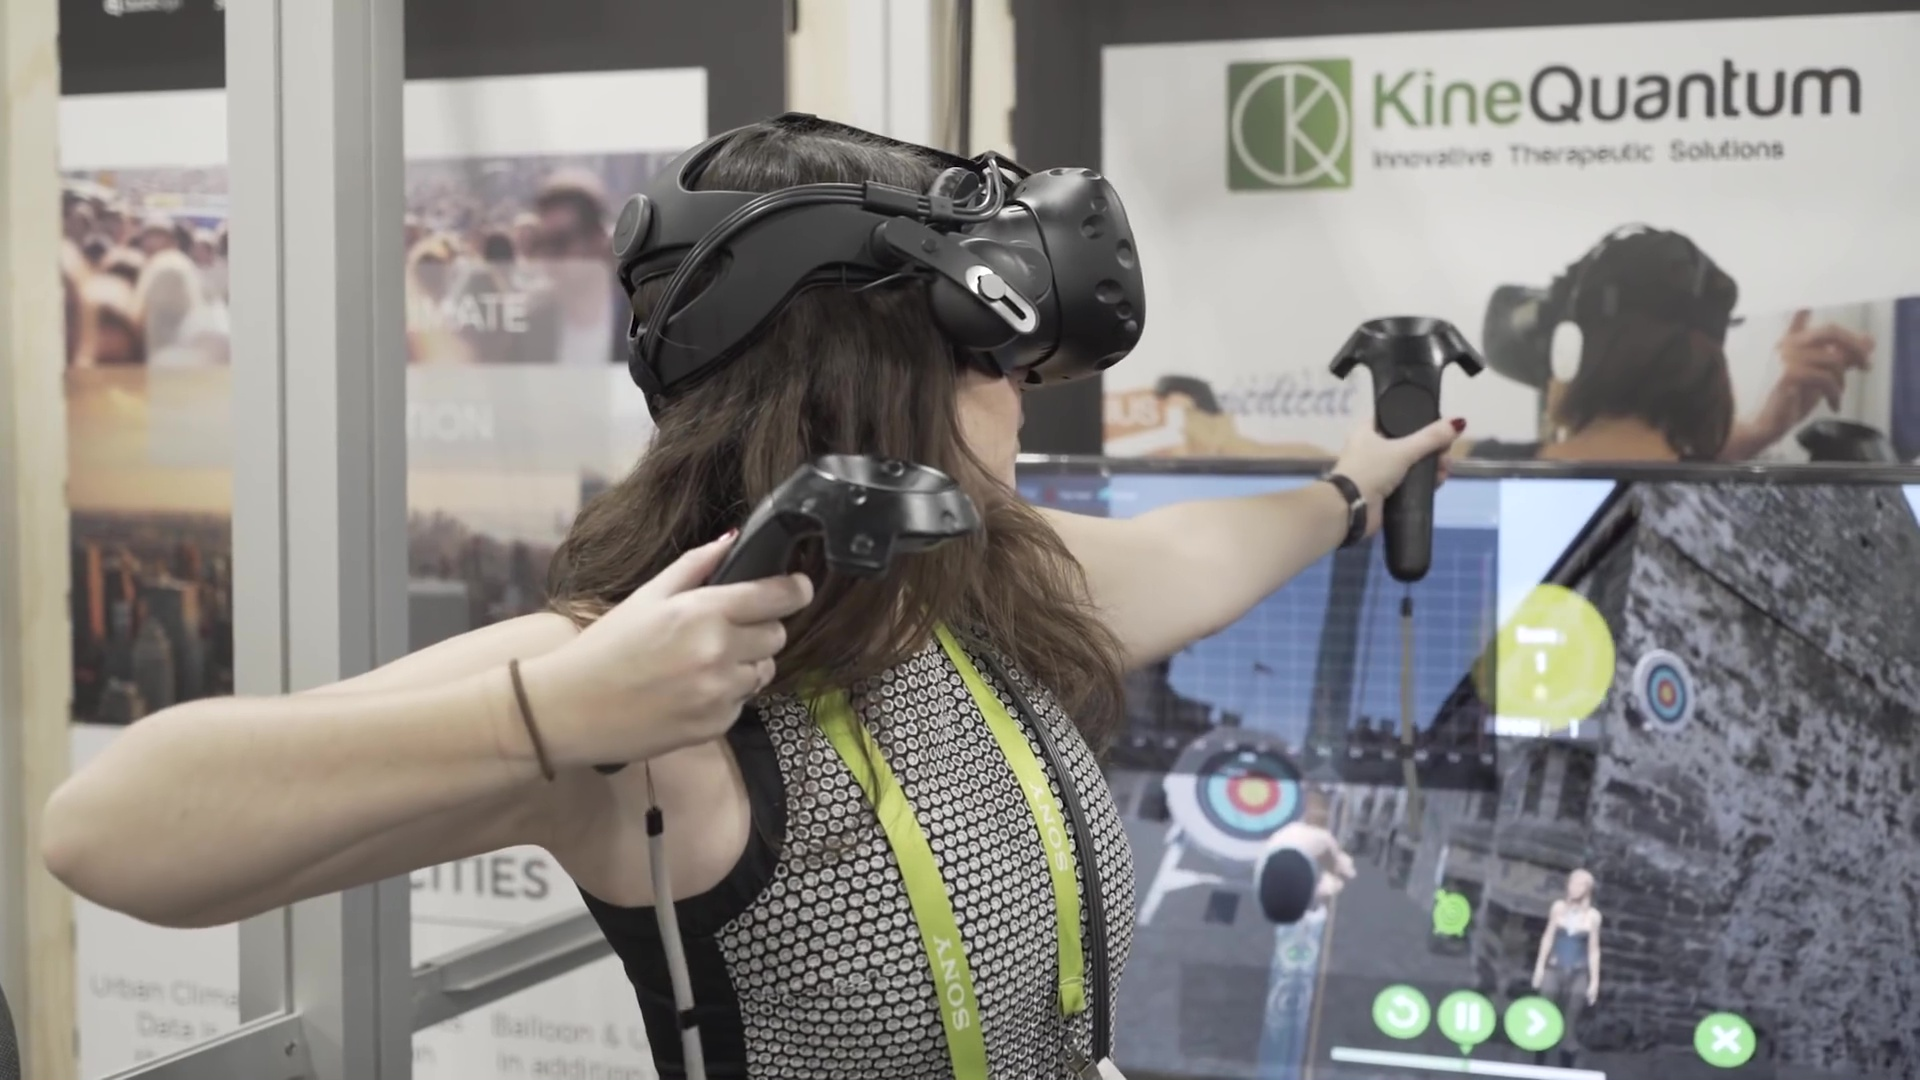
\includegraphics[scale=0.15]{kinequantum.jpg}
    \caption{Gebruiker van KineQuantum met de Htc Vive \autocite{Bergmann2018}}
\end{figure}
